%!TEX root =  ../paper.tex


\section{\name}
\label{sec:systemDesignMain}

Our goal is to design a solution that addresses the above limitations of previous solutions. In short, our solution should be \emph{secure} (no TOFU assumption, small TCB, no online authorities) and \emph{easy to deploy} (no OS re-installation, manual configuration or pre-defined enclaves). In this section, we provide an overview of our approach, outline possible use cases, describe our solution in detail and analyze its security.

\subsection{Approach Overview}

We propose a hardened SGX attestation scheme, called \name, based on a simple embedded device that we call \device. The embedded device is attached to the target platform over a local communication interface such as USB. 

% as shown in  Figure~\ref{fig:approach}. %Using this approach, we propose a hardened attestation mechanism to address the relay attacker defined in Section~\ref{sec:problemStatement:attackerModel}.

Our main idea is to use the combination of such trusted device and \emph{proximity verification} to prevent relay attacks. In our solution, the \device device verifies the proximity of the attested enclave and after successful proximity verification it facilitates the creation of a secure channel between the remote verifier and the attested enclave. 

After the initial attestation, the device periodically checks proximity to the attested enclave. The established secure channel is contingent on the physical presence of the embedded device on the target machine and it stays active only as long as the device is plugged-in. The act of detaching the device automatically revokes the attested platform without any interaction with a trusted authority. Thus, our solution enables secure \emph{offline} enrollment and revocation. 

To use our solution, enclave developers use a simple API that facilitates communications between the enclave and the device. 


\myparagraph{Security assumptions.}
%\label{sec:ext-adversary-model}
In our solution, the \device device is a trusted component. We deem this choice reasonable since it implements only the strictly necessary functions and therefore it a has significantly smaller software TCB, attack surface, and complexity compared to a general-purpose commodity OS. We assume that its issuer certifies each embedded device prior to its deployment and such certification can take place fully offline.

Concerning the security of the \device device we employ the same adversary model introduced in Section~\ref{sec:problemStatement} for enclaves. While the user's device and its private keys are never exposed to the attacker, another similar device can be in the physical possession of the attacker, which has as much time as she wants to fully compromise it (run arbitrary code and extract keys). 


\subsection{Example Use Cases}
\label{sec:use-cases}

Our solution is targeted to scenarios where the benefits of more secure attestation outweigh the deployment cost of a simple embedded device. Here, we outline three example cases.  

\myparagraph{Data center.} In our first example, we consider a cloud platform provider that attaches \device to a server in a specific data center and makes the public key of the connected device known to the users of the service. Our approach is particularly well suited to cloud computing models where customers rent dedicated computing resources like entire servers. In such a setting, our solution ensures that the cloud platform customer outsources data and computation to a server that resides in a specified location. Enforcing location may be desirable to meet increasing data protection regulation that defines how and where data can be stored, even if protected by TEEs such as SGX. Revocation (e.g., when a server is relocated to another data center or function) can be realized by merely detaching \device.

\myparagraph{Permissioned blockchain.} Our second case is a setting in which a trusted authority initializes a set of validator nodes for a permissioned and SGX-hardened blockchain. 
The trusted authority issues one \device for each organization that operates one of the validator nodes which allows secure attestation of the validator platforms. Organizations are free to upgrade their computing platforms by attaching the \device to a new platform which automatically revokes the old platform without the need to interact with a trusted authority. Furthermore, since \device can only be active on one platform at the time, such a deployment enables the authority to control the identities used in (Byzantine) blockchain consensus process.



\myparagraph{HSM-protected keys.} Our last case is the management of HSM-protected keys from an attested enclave. Such deployment enables the secure and flexible realization of various access control policies, implemented as attested enclaves. \name guarantees that only an enclave in the proximity of the HSM can control its keys. Such solution provides a high level of protection because, at no point in time, the HSM keys are directly accessible by the enclave (which may be vulnerable to side-channel attacks) or by the untrusted OS.


\subsection{Solution Details}
\label{sec:systemDesign}


Now, we explain the \name attestation mechanism in detail.


\myparagraph{I. Attestation protocol.} Figure~\ref{fig:systemSetUp} illustrates the attestation protocol that proceeds as follows:


\begin{figure}[t]
 \centering
  %\includegraphics[trim={0 4.6cm 18cm 0},clip,width=0.5\linewidth]{SystemSetupRevised_3.pdf}
  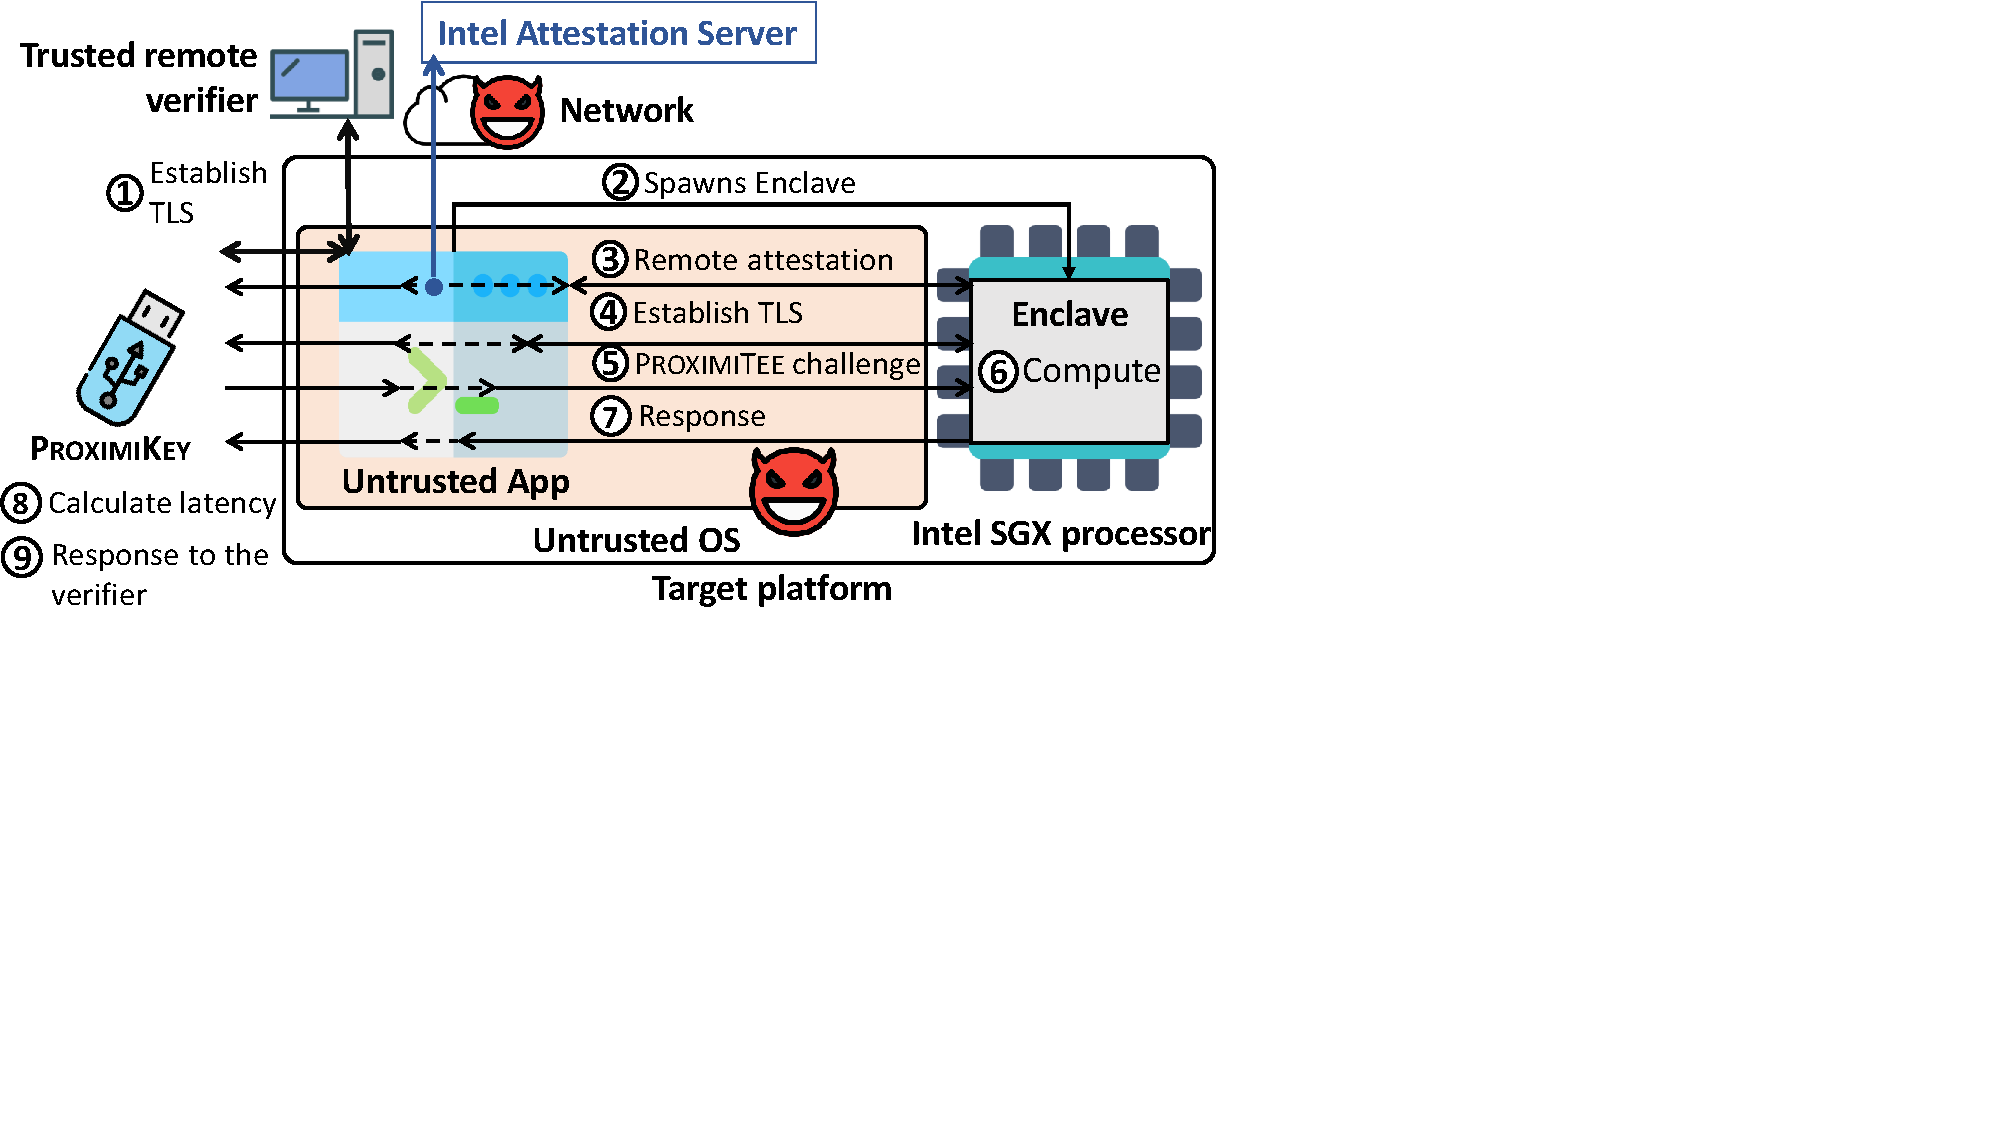
\includegraphics[trim={0 8.7cm 13.2cm 0},clip,width=\linewidth]{proximiteeMain.pdf}
 \caption{\textbf{\name attestation.} The remote verifier establishes a secure channel to the \device device that first attests the enclave and then verifies its proximity.}
 	\label{fig:systemSetUp}
 	\figsaverL
\end{figure}

\begin{mylist}
  \item[\one] The remote verifier establishes a secure channel (e.g., \tls) to the certified \device. An assisting but untrusted user-space application facilitates the connection on the target platform acting as a transport channel between the remote verifier and the \device (and later also the enclave). As part of this first step, the remote verifier specifies which enclave should be executed.

  \item[\two] The untrusted application creates and starts the attestation target enclave.

  \item[\three] \device performs the standard remote attestation to verify the code configuration of the enclave with the help of the IAS server or using a custom DCAP procedure (see Section~\ref{sec:background}). In the attestation protocol, the device learns the public key of the attested enclave.

  \item[\four] \device establishes a secure channel (e.g., \tls) to the enclave using that public key.

  \item[\five] \device performs a distance-bounding protocol that consists of $n$ rounds, where each round is formed by steps \five to \eight.
  %(see Figure~\ref{fig:challengeResponse}).
  At the beginning of each round \device generates a random challenge $r$ and sends it to the enclave over the TLS channel.

  \item[\six] The enclave increments the received challenge by one $(r+1)$.

  \item[\seven] The enclave sends a response ($r+1$) back to the \device over the \tls channel.

  \item[\eight] \device verifies that the response value is as expected (i.e., $r+1$) and checks if the latency of the response is below a threshold (\connect). Successful proximity verification requires that the latency is below the threshold for at least $k \times n$ responses, where $k \in (0, 1]$ is a percentage of the total number of responses $n$.

  \item[\nine] If proximity verification is successful, the \device notifies the remote verifier over the \tls channel (constructed in step \one). The verifier starts using the \device TLS channel to send messages to the enclave.
\end{mylist}


\myparagraph{II. Periodic proximity verification.} After the initial connection establishment, the \device device performs \emph{periodic} proximity verification on the attested enclave. \device sends a new random challenge $r$ at frequency $f$, verifies the correctness of the received response and measures its latency. The latest $w$ latencies are stored to a sliding window data structure, as shown in Figure~\ref{fig:slidingWindow}.

\begin{figure}[t]
  \centering
    %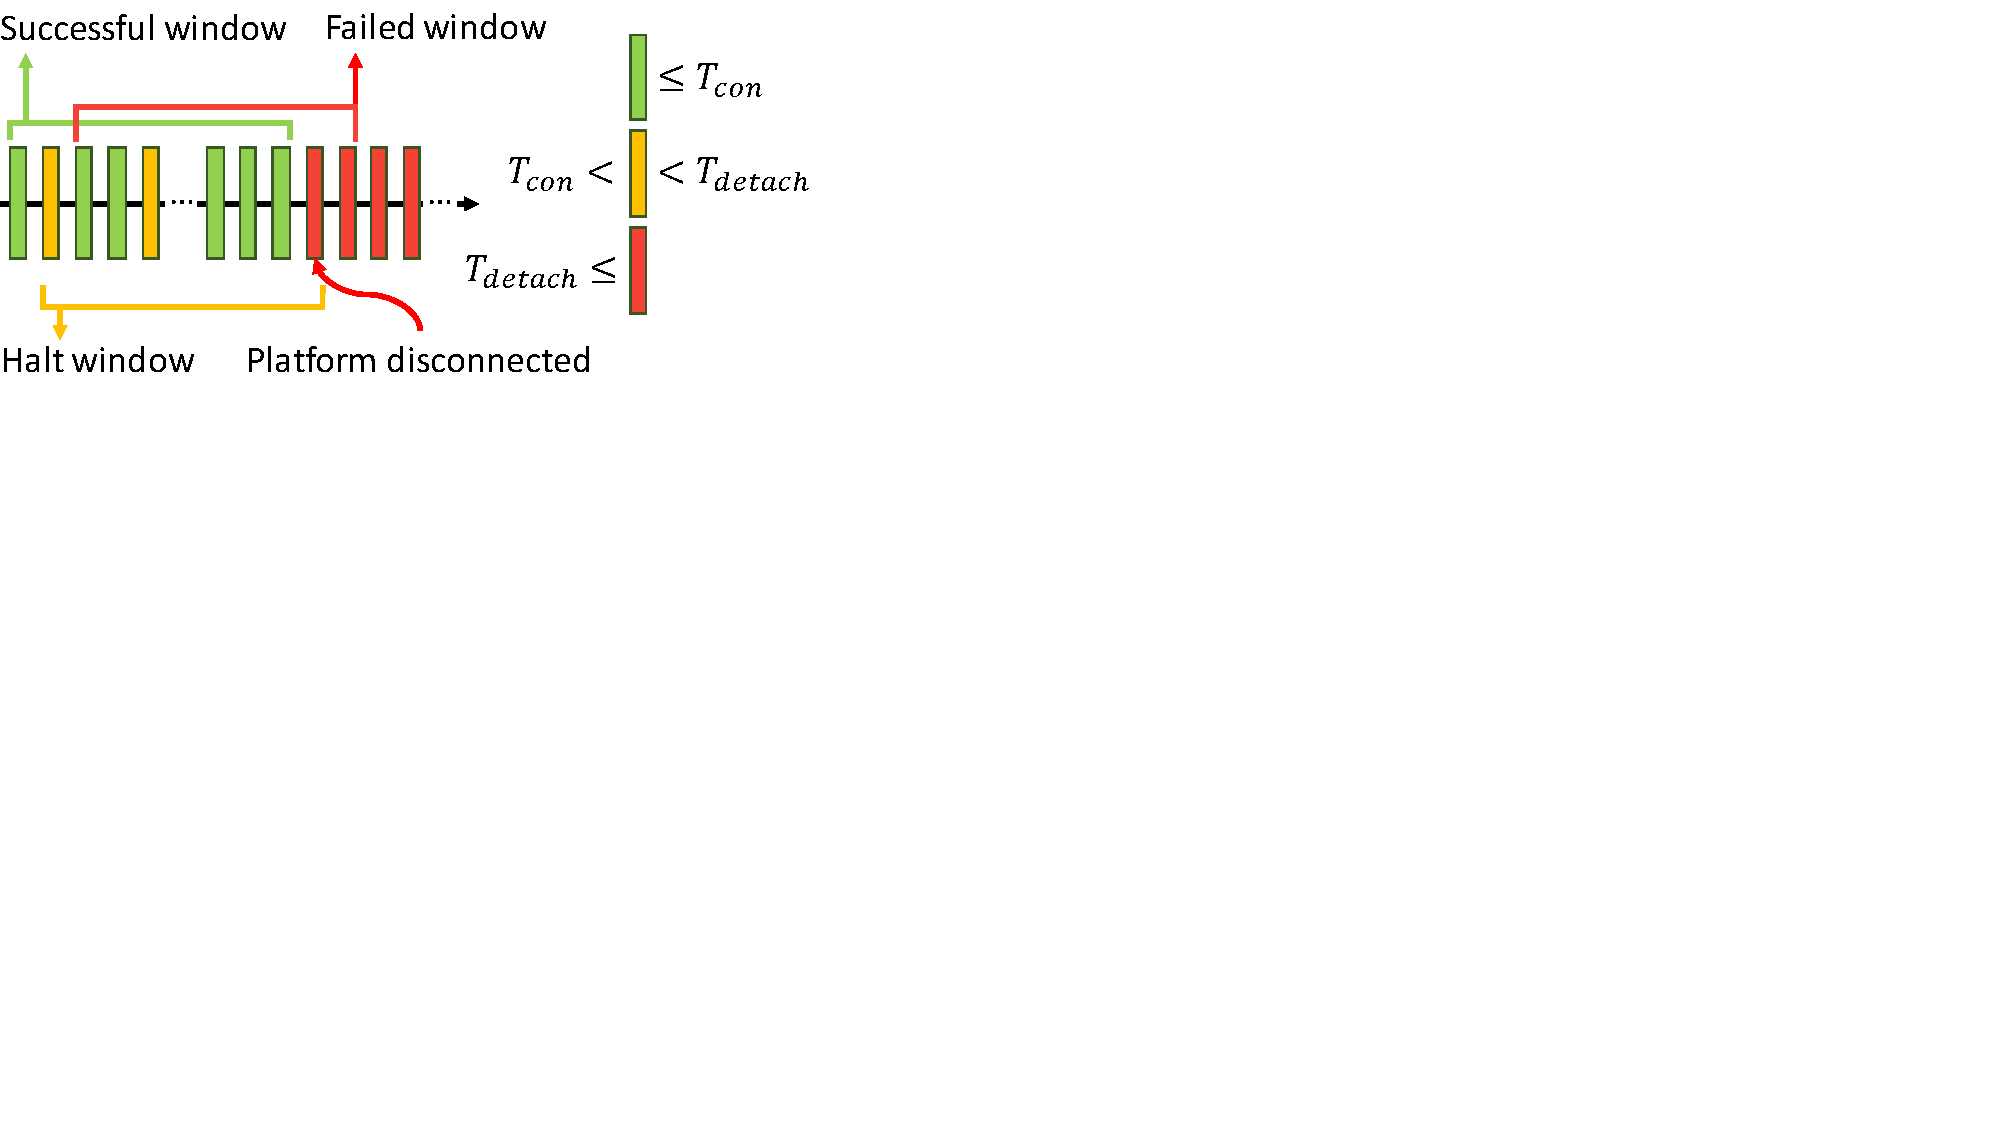
\includegraphics[trim={0 12.7cm 20cm 0}, clip, width=0.65\linewidth]{SlidingWindow.pdf}
    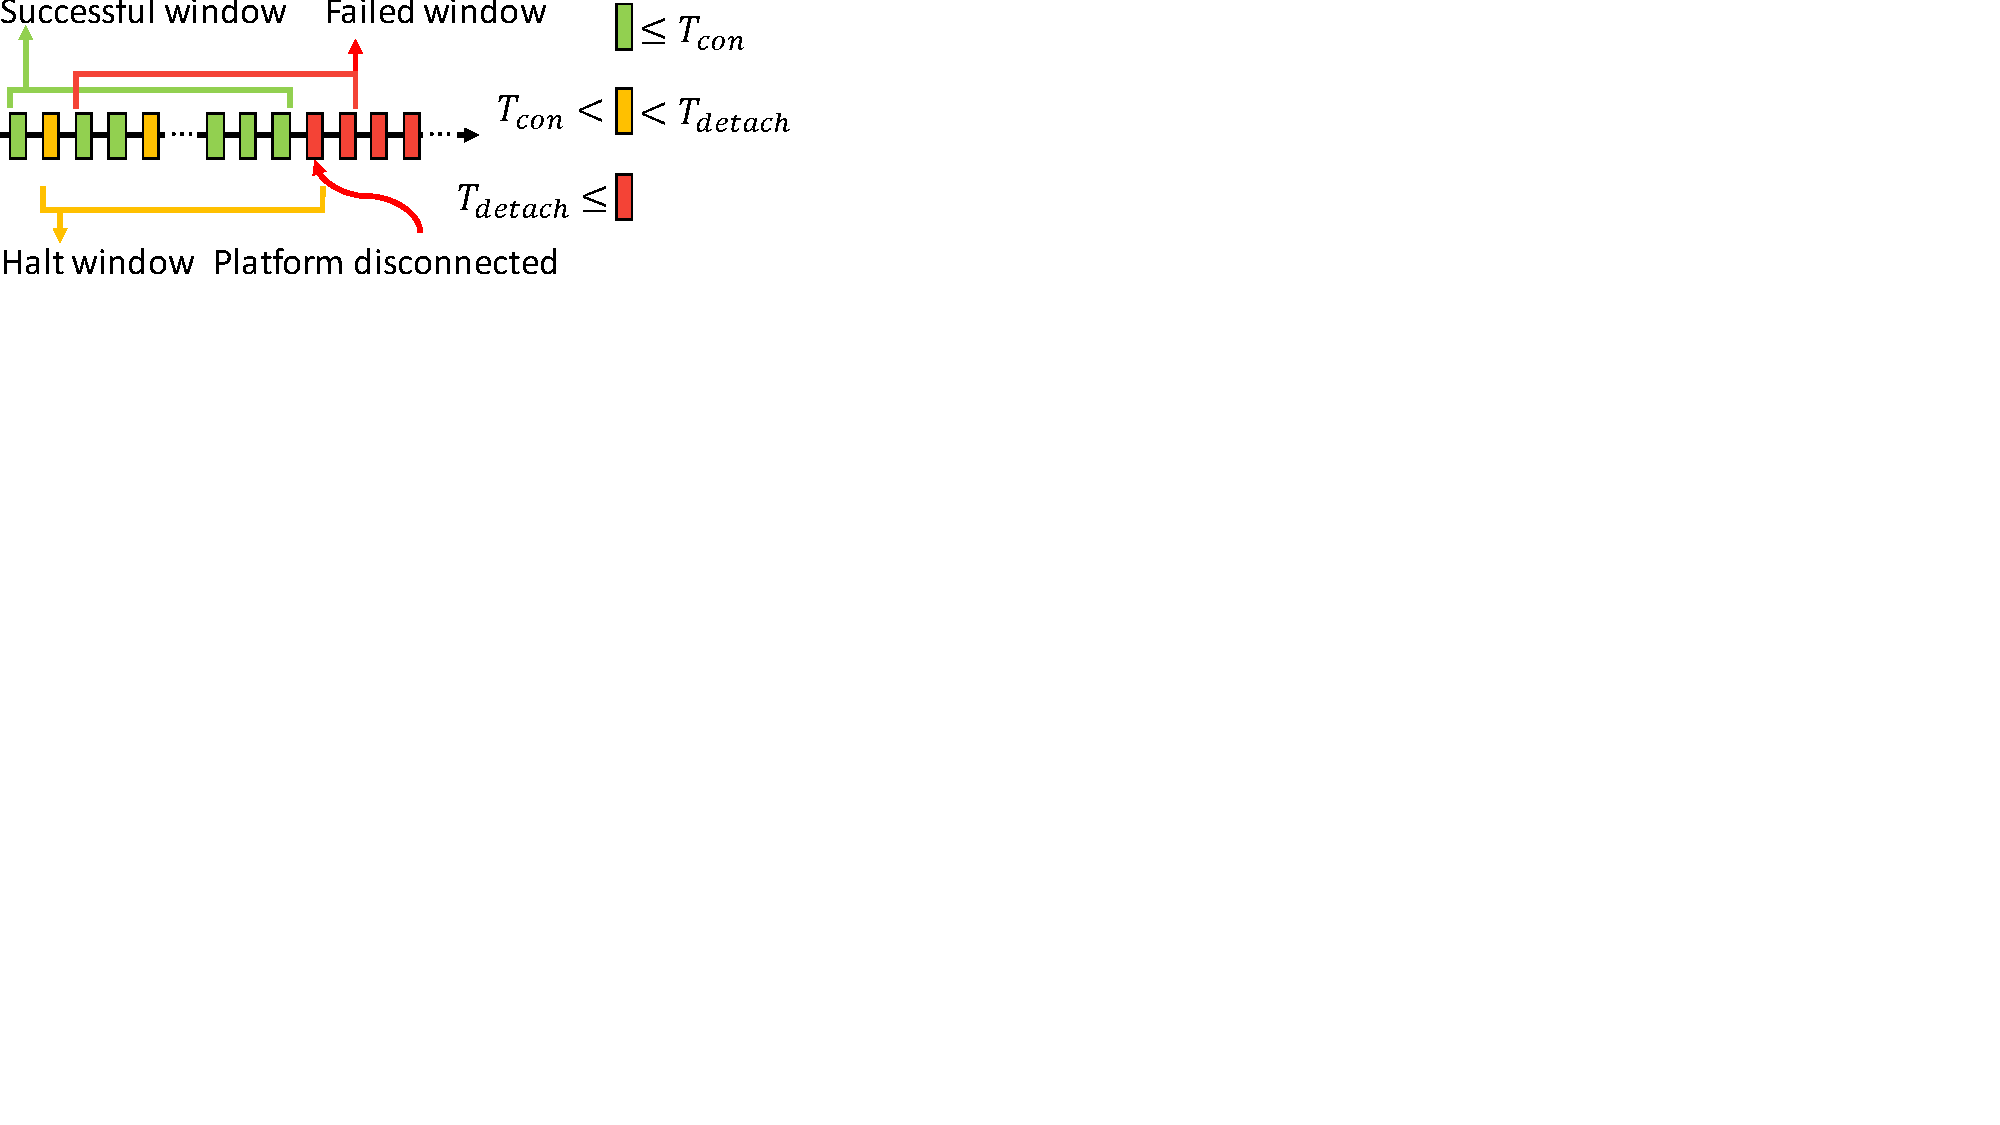
\includegraphics[trim={0 14cm 20cm 0}, clip, width=0.7\linewidth]{SlidingWindow_1.pdf}
    \caption{\textbf{Sliding window} for periodic proximity verification with three different types of challenge-response latencies.}
    \figsaver
    \label{fig:slidingWindow}
\end{figure}

As elaborated in Section~\ref{sec:evaluation} there are three types of latencies in the presence of relay attacks. The first type of response is received faster than the  threshold \connect (green in Figure~\ref{fig:slidingWindow}), these responses can only be produced if no attack is taking place. In the second type of response the latency exceeds \connect, but it is below another, higher threshold \detach (yellow), these are sometimes observed during legitimate connections and sometimes during relay attacks. And third, the latency is equal to or exceeds \detach (red), these latencies are only observed while a relay attack is being performed. Given such a sliding window of periodic challenge-response latencies, we define the following rules for halting or terminating the connection:

\begin{mylist_indent}
  \item \emph{Successful window: no action.} If at least $k$ responses have latency $\leq$\connect and none of the response have latency$\geq$\detach, the current window legitimate and \device keeps the connection active.
 
  \item \emph{Halt window: prevent communication.} If one of the responses have latency $\geq$\detach, we consider the current window a ``halt window,'' and \device stops forwarding data to the enclave until the current window is legitimate again.

  \item \emph{Failed window: terminate channel.} If two or more responses have latencies $\geq$\detach, we consider the current window a ``failed window'' and \device terminates the communication and thus revokes the attested platform.
\end{mylist_indent}




\subsection{Security Analysis}

\noindent\textbf{Attestation security.}
To analyze the security of our hardened attestation mechanism, we must first define successful attestation. We say that the attestation is successful when the remote verifier establishes a connection to the correct enclave that i) has the expected code measurement and ii) runs on the computing platform to which the \device device is attached.


The task of establishing a secure channel to the correct enclave can be broken into two subtasks. The first subtask is to establish a secure channel to the correct \device device. This is achieved using standard device certification. We assume that the adversary cannot compromise the specific \device used. If the adversary manages to extract keys from other \device devices, he cannot trick the remote verifier to connect to a wrong enclave, as the remote verifier will only communicate with a pre-defined embedded device.




The second subtask is to establish a secure connection from \device to the correct enclave. For this, we use proximity verification. \device verifies the proximity of the attested enclave through steps \five to \eight of the protocol. These steps essentially check two things. First, through step \seven, whether the messages are received from the correct enclave. This verification is performed by checking the correctness of the decrypted message, and it relies on the assumption that the attacker cannot break the underlying encryption and hence only the enclave that has access to the key that was bound to the attestation could have produced a valid reply. Second, through step \eight, whether the \device and the enclave are in each other's proximity. This check relies on the assumption that a reply from a remote enclave will take more time to reach the \device than a reply from the local enclave.

We evaluate the second aspect experimentally. In particular, we simulate a powerful relay-attack adversary that is connected to the target platform with fast network connection. To consider the best case for the adversary, we make several assumptions in his favor. For example, we assume that he can instantly perform all computations needed to participate in the proximity verification protocol. However, he cannot break cryptographic hardness assumptions. We define the adversary's success as the event in which proximity verification succeeds with an enclave that resides on the attacker's platform and denote the probability of such event $P_{adv}$. We define the legitimate success as the event in which proximity verification succeeds with an enclave that resides in the target platform and denote its probability $P_{legit}$. In Section~\ref{sec:evaluation} we show that it is possible to find parameters ($n=50$, $k=0.3$ and \connect$=186 \mu s$) that make proximity verification very secure ($P_{adv}=3.55\times 10^{-34}$) and reliable ($P_{legit}=0.999999977$).



\parasaver
\myparagraph{Revocation security.}
To analyze the security of the periodic proximity verification which we use for platform revocation, we must first define what it means for the attacker to break the periodic proximity verification. The purpose of the periodic proximity verification is to prevent cases where the user detaches the \device device from the attested target platform and attaches it to another SGX platform before the previously established connection is terminated. Since we consider an adversary who does not have physical access to the target platform (recall Section~\ref{sec:problemStatement:systemAttackerModel}), we focus on benign users and exclude scenarios where the \device would be connected to multiple SGX platforms with custom wiring or rapidly and repeatedly plugged in and out of two SGX platforms.



We define the periodic proximity verification as broken if the adversary can manage to keep the previously established connection alive within a ``short delay'' after the \device was detached from the attested target platform. For most practical purposes we consider a delay of 10 ms as sufficiently short. We denote the adversary's success probability in breaking the periodic proximity verification as $P'_{adv}$.
%
A false positive for periodic attestation is the event where the connection to the legitimate enclave is terminated, and the attested platform is revoked despite the \device being connected to the target platform. We denote the probability that this happens during a ``long period'' as $P'_{fp}$. We consider an example period of 10 years sufficiently long for most practical deployments.

In Section~\ref{sec:evaluation} we experimentally shows that revocation can be secure ($P'_{avd}=3.55\times10^{-34}$) and reliable
($P'_{fp}=1.6\times10^{-4}$) while consuming only a minor fraction of the available channel capacity.


